%  LaTeX support: latex@mdpi.com
%  For support, please attach all files needed for compiling as well as the log file, and specify your operating system, LaTeX version, and LaTeX editor.

%=================================================================
% pandoc conditionals added to preserve backwards compatibility with previous versions of rticles

\documentclass[econometrics,article,submit,moreauthors,pdftex]{Definitions/mdpi}


%% Some pieces required from the pandoc template
\setlist[itemize]{leftmargin=*,labelsep=5.8mm}
\setlist[enumerate]{leftmargin=*,labelsep=4.9mm}


%--------------------
% Class Options:
%--------------------

%---------
% article
%---------
% The default type of manuscript is "article", but can be replaced by:
% abstract, addendum, article, book, bookreview, briefreport, casereport, comment, commentary, communication, conferenceproceedings, correction, conferencereport, entry, expressionofconcern, extendedabstract, datadescriptor, editorial, essay, erratum, hypothesis, interestingimage, obituary, opinion, projectreport, reply, retraction, review, perspective, protocol, shortnote, studyprotocol, systematicreview, supfile, technicalnote, viewpoint, guidelines, registeredreport, tutorial
% supfile = supplementary materials

%----------
% submit
%----------
% The class option "submit" will be changed to "accept" by the Editorial Office when the paper is accepted. This will only make changes to the frontpage (e.g., the logo of the journal will get visible), the headings, and the copyright information. Also, line numbering will be removed. Journal info and pagination for accepted papers will also be assigned by the Editorial Office.

%------------------
% moreauthors
%------------------
% If there is only one author the class option oneauthor should be used. Otherwise use the class option moreauthors.

%---------
% pdftex
%---------
% The option pdftex is for use with pdfLaTeX. Remove "pdftex" for (1) compiling with LaTeX & dvi2pdf (if eps figures are used) or for (2) compiling with XeLaTeX.

%=================================================================
% MDPI internal commands - do not modify
\firstpage{1}
\makeatletter
\setcounter{page}{\@firstpage}
\makeatother
\pubvolume{1}
\issuenum{1}
\articlenumber{0}
\pubyear{2023}
\copyrightyear{2023}
%\externaleditor{Academic Editor: Firstname Lastname}
\datereceived{ }
\daterevised{ } % Comment out if no revised date
\dateaccepted{ }
\datepublished{ }
%\datecorrected{} % For corrected papers: "Corrected: XXX" date in the original paper.
%\dateretracted{} % For corrected papers: "Retracted: XXX" date in the original paper.
\hreflink{https://doi.org/} % If needed use \linebreak
%\doinum{}
%\pdfoutput=1 % Uncommented for upload to arXiv.org

%=================================================================
% Add packages and commands here. The following packages are loaded in our class file: fontenc, inputenc, calc, indentfirst, fancyhdr, graphicx, epstopdf, lastpage, ifthen, float, amsmath, amssymb, lineno, setspace, enumitem, mathpazo, booktabs, titlesec, etoolbox, tabto, xcolor, colortbl, soul, multirow, microtype, tikz, totcount, changepage, attrib, upgreek, array, tabularx, pbox, ragged2e, tocloft, marginnote, marginfix, enotez, amsthm, natbib, hyperref, cleveref, scrextend, url, geometry, newfloat, caption, draftwatermark, seqsplit
% cleveref: load \crefname definitions after \begin{document}

%=================================================================
% Please use the following mathematics environments: Theorem, Lemma, Corollary, Proposition, Characterization, Property, Problem, Example, ExamplesandDefinitions, Hypothesis, Remark, Definition, Notation, Assumption
%% For proofs, please use the proof environment (the amsthm package is loaded by the MDPI class).

%=================================================================
% Full title of the paper (Capitalized)
\Title{El espejismo del PIB y la trampa turística: presión inmobiliaria
en las provincias españolas}

% MDPI internal command: Title for citation in the left column
\TitleCitation{El espejismo del PIB y la trampa turística: presión
inmobiliaria en las provincias españolas}

% Author Orchid ID: enter ID or remove command
%\newcommand{\orcidauthorA}{0000-0000-0000-000X} % Add \orcidA{} behind the author's name
%\newcommand{\orcidauthorB}{0000-0000-0000-000X} % Add \orcidB{} behind the author's name


% Authors, for the paper (add full first names)
\Author{Rubén Sánchez Munuera$^{1,*}$, Luis Molina Villar$^{1,*}$, Pablo
Gallart Carbonell$^{1,*}$}


%\longauthorlist{yes}


% MDPI internal command: Authors, for metadata in PDF
\AuthorNames{Rubén Sánchez Munuera, Luis Molina Villar, Pablo Gallart
Carbonell}

% MDPI internal command: Authors, for citation in the left column
%\AuthorCitation{Lastname, F.; Lastname, F.; Lastname, F.}
% If this is a Chicago style journal: Lastname, Firstname, Firstname Lastname, and Firstname Lastname.
\AuthorCitation{Sánchez Munuera, R.; Molina Villar, L.; Gallart
Carbonell, P.}

% Affiliations / Addresses (Add [1] after \address if there is only one affiliation.)
\address{%
$^{1}$ \quad Máster en Ciencia de Datos, Universitat de València,
España; \\
}

% Contact information of the corresponding author
\corres{Correspondence: }

% Current address and/or shared authorship








% The commands \thirdnote{} till \eighthnote{} are available for further notes

% Simple summary

%\conference{} % An extended version of a conference paper

% Abstract (Do not insert blank lines, i.e. \\)
\abstract{El PIB per cápita provincial se utiliza como medida de
prosperidad, pero puede desconectarse del coste de la vivienda en los
territorios donde la demanda no depende de la renta local. Este trabajo
analiza esa desconexión en las 52 provincias y ciudades autónomas
españolas en 2022. Definimos un índice de presión inmobiliaria (valor
medio de las transacciones de vivienda libre dividido por el PIB per
cápita) y lo relacionamos con el peso de los servicios (comercio,
transporte, hostelería, información y comunicaciones) y de la industria
en el valor añadido bruto, con datos del INE y del Ministerio de
Vivienda. Aplicamos análisis univariante y bivariante, correlaciones de
Spearman y pruebas de robustez. El PIB per cápita se asocia débilmente
con el valor de la vivienda (correlación de 0,29) y no
significativamente con la presión inmobiliaria. Esta se asocia
positivamente con el peso de los servicios (0,49) y negativamente con el
de la industria (−0,56), y ambas asociaciones resisten la exclusión de
provincias singulares; sin embargo, al controlar por la industria, la de
los servicios deja de ser significativa. Los resultados, transversales y
descriptivos, no permiten atribuir la presión a la especialización
turística en sentido estricto.}


% Keywords
\keyword{espejismo del PIB; presión inmobiliaria; precio de la vivienda;
estructura productiva; provincias españolas; correlación de Spearman}

% The fields PACS, MSC, and JEL may be left empty or commented out if not applicable
%\PACS{J0101}
%\MSC{}
%\JEL{}

%%%%%%%%%%%%%%%%%%%%%%%%%%%%%%%%%%%%%%%%%%
% Only for the journal Diversity
%\LSID{\url{http://}}

%%%%%%%%%%%%%%%%%%%%%%%%%%%%%%%%%%%%%%%%%%
% Only for the journal Applied Sciences

%%%%%%%%%%%%%%%%%%%%%%%%%%%%%%%%%%%%%%%%%%

%%%%%%%%%%%%%%%%%%%%%%%%%%%%%%%%%%%%%%%%%%
% Only for the journal Data



%%%%%%%%%%%%%%%%%%%%%%%%%%%%%%%%%%%%%%%%%%
% Only for the journal Toxins


%%%%%%%%%%%%%%%%%%%%%%%%%%%%%%%%%%%%%%%%%%
% Only for the journal Encyclopedia


%%%%%%%%%%%%%%%%%%%%%%%%%%%%%%%%%%%%%%%%%%
% Only for the journal Advances in Respiratory Medicine
%\addhighlights{yes}
%\renewcommand{\addhighlights}{%

%\noindent This is an obligatory section in “Advances in Respiratory Medicine”, whose goal is to increase the discoverability and readability of the article via search engines and other scholars. Highlights should not be a copy of the abstract, but a simple text allowing the reader to quickly and simplified find out what the article is about and what can be cited from it. Each of these parts should be devoted up to 2~bullet points.\vspace{3pt}\\
%\textbf{What are the main findings?}
% \begin{itemize}[labelsep=2.5mm,topsep=-3pt]
% \item First bullet.
% \item Second bullet.
% \end{itemize}\vspace{3pt}
%\textbf{What is the implication of the main finding?}
% \begin{itemize}[labelsep=2.5mm,topsep=-3pt]
% \item First bullet.
% \item Second bullet.
% \end{itemize}
%}


%%%%%%%%%%%%%%%%%%%%%%%%%%%%%%%%%%%%%%%%%%


% tightlist command for lists without linebreak
\providecommand{\tightlist}{%
  \setlength{\itemsep}{0pt}\setlength{\parskip}{0pt}}



\DeclareUnicodeCharacter{2212}{-}
\DeclareUnicodeCharacter{03C1}{$\rho$}
\usepackage{longtable}
\usepackage{booktabs}
\usepackage{array}
\usepackage{multirow}
\usepackage{wrapfig}
\usepackage{float}
\usepackage{colortbl}
\usepackage{pdflscape}
\usepackage{tabularx}
\usepackage{xltabular}
\usepackage{threeparttable}
\usepackage{threeparttablex}
\usepackage[normalem]{ulem}
\usepackage{makecell}
\usepackage{xcolor}

\begin{document}



%%%%%%%%%%%%%%%%%%%%%%%%%%%%%%%%%%%%%%%%%%

\section{Introducción}\label{introducciuxf3n}

El producto interior bruto (PIB) per cápita es la medida más habitual de
la prosperidad de un territorio. Sin embargo, el PIB provincial mide la
actividad que se produce en cada provincia, no necesariamente la renta
de las personas que viven en ella. En territorios donde buena parte de
la actividad se vincula al turismo, la segunda residencia o la demanda
de no residentes, el precio de la vivienda puede quedar determinado por
una demanda que no depende del PIB que generan sus habitantes. A esta
posible desconexión entre la riqueza medida y el coste de acceder a una
vivienda la denominamos aquí ``el espejismo del PIB''.

Este trabajo estudia esa desconexión en las 52 provincias y ciudades
autónomas de España en 2022. Para ello definimos un índice de presión
inmobiliaria, el cociente entre el valor medio de las transacciones de
vivienda libre y el PIB per cápita provincial, y lo cruzamos con la
estructura productiva. Nuestra pregunta central es si las provincias
cuya riqueza se apoya más en el comercio, el transporte y la hostelería
soportan una presión inmobiliaria mayor que las de mayor peso
industrial. Planteamos dos hipótesis de trabajo: una asociación positiva
entre el peso de los servicios y la presión inmobiliaria, y una
asociación negativa con el peso de la industria. Se trata de hipótesis
sobre asociaciones, y el diseño transversal del estudio no permite
establecer relaciones causales.

El resto del artículo se organiza así. La sección de datos y métodos
describe las fuentes del Instituto Nacional de Estadística (INE) y del
Ministerio de Vivienda, la construcción del índice y el tratamiento de
valores perdidos y atípicos. La sección de resultados presenta el
análisis univariante y bivariante y comprueba su robustez. Cerramos con
una discusión de las limitaciones y las conclusiones sobre las dos
preguntas planteadas.

\section{Datos y métodos}\label{datos-y-muxe9todos}

\subsection{Fuentes de datos y año de
referencia}\label{fuentes-de-datos-y-auxf1o-de-referencia}

Para la realización de este análisis y la contrastación de nuestra
hipótesis sobre el impacto del sector servicios en el mercado
inmobiliario, se ha optado por realizar un análisis de corte transversal
(\emph{cross-sectional}) centrado en el ejercicio fiscal 2022. Esta
decisión metodológica se fundamenta en tres criterios operativos:

\emph{Efecto estabilizador post-pandemia.} Los años 2020 y 2021
presentan anomalías extremas en la Contabilidad Regional debido a las
restricciones de movilidad y la paralización de la hostelería derivadas
de la COVID-19. Incluir estos años distorsionaría el análisis
estructural de las provincias dependientes del turismo. 2022 representa
el primer ejercicio de reactivación económica normalizada.

\emph{Consolidación estadística.} En las series publicadas por el
Instituto Nacional de Estadística (INE), los datos correspondientes a
2023 y 2024 figuran bajo las etiquetas de ``Avance (A)'' o ``Provisional
(P)''. El año 2022 garantiza el uso de cifras definitivas y consolidadas
tanto en el PIB como en el Valor Añadido Bruto sectorial.

\emph{Claridad analítica y espacial.} Dada la limitación de extensión
del informe, un análisis de corte transversal permite generar
visualizaciones bivariantes nítidas (diagramas de dispersión de 52
observaciones) que muestran la correlación estructural actual, evitando
el solapamiento o ``ruido'' visual que generaría la representación de
series temporales completas.

La Tabla \ref{tab:tabvars} resume las variables empleadas y su origen.

\begin{table}[H]

\caption{\label{tab:tabvars}Variables utilizadas en el análisis (52 provincias y ciudades autónomas, 2022).}
\centering
\begin{tabular}[t]{l>{\raggedright\arraybackslash}p{5cm}>{\raggedright\arraybackslash}p{3.3cm}}
\toprule
Variable & Descripción & Fuente\\
\midrule
PIB\_per\_capita & PIB per cápita provincial, 2022 (euros) & INE, pr\_cre\_26.xls\\
pct\_industria & Peso de la industria (ramas B-E: extractivas, manufacturera, energía, agua y residuos) en el VAB total, 2022 (\%) & INE, 77776.xlsx\\
pct\_servicios\_turismo & Peso de comercio, transporte, hostelería e información y comunicaciones (rama G-J) en el VAB total, 2022 (\%) & INE, 77776.xlsx\\
Valor\_Vivienda\_2022 & Valor medio de las transacciones de vivienda libre, media de los cuatro trimestres de 2022 (euros) & Ministerio de Vivienda, 34020150.csv\\
presion\_inmobiliaria & Cociente entre el valor medio de la vivienda y el PIB per cápita (adimensional) & Elaboración propia\\
\bottomrule
\end{tabular}
\end{table}

\subsection{Importación y limpieza}\label{importaciuxf3n-y-limpieza}

\subsubsection{PIB per cápita (2022)}\label{pib-per-cuxe1pita-2022}

El PIB per cápita provincial procede de la Contabilidad Regional de
España (INE, Revisión Estadística 2024). Del fichero se conservaron las
52 provincias y ciudades autónomas, descartando los totales nacionales,
los agregados de comunidades pluriprovinciales y las notas al pie, y se
armonizaron los nombres con los de las otras fuentes.

\subsubsection{Estructura productiva (VAB por
sectores)}\label{estructura-productiva-vab-por-sectores}

El archivo original del INE presenta una estructura orientada a la
visualización humana, mezclando dos niveles jerárquicos distintos en la
misma columna. En la columna principal se intercala el nombre de la
provincia (ej. ``02 Albacete'') con celdas de datos vacías, seguido en
las filas inferiores de los sectores productivos (ej. ``A.
Agricultura'') con sus valores correspondientes. Si importamos esto de
forma directa, la conexión relacional entre cada sector y su provincia
se perdería, invalidando el análisis. Para resolverlo aplicamos una
técnica de reestructuración (\emph{data wrangling}):

\begin{enumerate}
\def\labelenumi{\arabic{enumi}.}
\tightlist
\item
  Condicional \texttt{if\_else} + expresión regular: detecta códigos
  numéricos iniciales para identificar qué filas actúan como ``cabecera
  de provincia''.
\item
  Función \texttt{fill(.direction\ =\ "down")}: arrastra el nombre de la
  provincia detectada hacia todas las filas de sus sectores.
\item
  Expresiones regulares: simplifican la verbosidad de los nombres
  sectoriales.
\item
  Pivotaje (\texttt{pivot\_wider}): transforma la estructura a formato
  \emph{tidy}, donde cada provincia es una fila única y cada sector una
  variable (columna).
\end{enumerate}

\subsubsection{Precio medio de la vivienda
(2022)}\label{precio-medio-de-la-vivienda-2022}

Los archivos de transacciones inmobiliarias del Ministerio de Vivienda
(34020150\ldots csv) presentan dos complejidades técnicas importantes
que debemos resolver con rigor analítico.

\emph{Estructura trimestral frente a anual.} El archivo desglosa el
precio medio por cada trimestre (T1, T2, T3, T4) para cada año. Para
cruzarlo con el PIB y el VAB (que son anuales en el año 2022) no podemos
coger un único trimestre al azar, ya que introduciría un sesgo
estacional (por ejemplo, el precio en zonas turísticas varía mucho entre
verano e invierno). Lo metodológicamente riguroso es calcular la media
aritmética de los cuatro trimestres del año 2022 para obtener el precio
medio anual representativo.

\emph{Formato numérico español.} Los valores monetarios vienen en
formato de texto con puntos para los miles y comas para los decimales
(ej. ``183.747,9''). Si R los lee tal cual, los interpretará como
carácter. Debemos limpiar las cadenas de texto y convertirlas a formato
numérico continuo (\texttt{numeric}).

\subsection{Índice de presión
inmobiliaria}\label{uxedndice-de-presiuxf3n-inmobiliaria}

El índice de presión inmobiliaria de cada provincia es el cociente entre
el valor medio de las transacciones de vivienda libre y su PIB per
cápita. Es adimensional y se interpreta como el número de PIB per cápita
anuales al que equivale una vivienda media: un valor de 5 indica que la
vivienda media cuesta cinco veces lo que se produce por habitante en un
año.

\subsection{Valores perdidos y
atípicos}\label{valores-perdidos-y-atuxedpicos}

\subsubsection{Valores perdidos}\label{valores-perdidos}

Las tres fuentes se unieron por el nombre de la provincia, tras
armonizar las denominaciones (por ejemplo, ``Madrid, Comunidad de'' y
``Madrid (Comunidad de)'' pasan a ``Madrid''). El conjunto final
contiene \text{52} observaciones y \text{0} valores perdidos en el
conjunto de variables analizadas. Todas las provincias con PIB per
cápita disponen también de estructura productiva y de precio de la
vivienda, de modo que ninguna observación quedó sin cruzar.

\textbf{Decisión:} al no haber valores perdidos, no se imputa ni se
elimina ninguna provincia. Este punto es relevante, porque con solo 52
observaciones cada exclusión alteraría de forma apreciable los
resultados.

\subsubsection{Valores atípicos}\label{valores-atuxedpicos}

Para identificar valores atípicos aplicamos el criterio de Tukey: se
considera atípica una provincia cuyo valor queda por encima de Q3 +
1,5·RIC o por debajo de Q1 − 1,5·RIC, donde RIC es el rango
intercuartílico. Previamente se comprobó que todos los valores son
coherentes (porcentajes entre 0 y 100, precios y PIB positivos), de modo
que ninguno responde a un error de importación. La Tabla
\ref{tab:tabatipicos} recoge las provincias señaladas y la Figura
\ref{fig:atipicos} su posición en la distribución.

\begin{table}[H]

\caption{\label{tab:tabatipicos}Provincias atípicas según el criterio de Tukey (1,5 veces el rango intercuartílico).}
\centering
\begin{tabular}[t]{llrr}
\toprule
Variable & Provincia & Valor & Valla superada\\
\midrule
Presión inmobiliaria & Balears, Illes & 12,98 & 9,58\\
Presión inmobiliaria & Málaga & 12,82 & 9,58\\
Servicios, rama G-J (\%) & Balears, Illes & 37,09 & 33,18\\
Servicios, rama G-J (\%) & Palmas, Las & 36,08 & 33,18\\
Servicios, rama G-J (\%) & Madrid & 33,61 & 33,18\\
\bottomrule
\end{tabular}
\end{table}

\begin{figure}[H]

{\centering 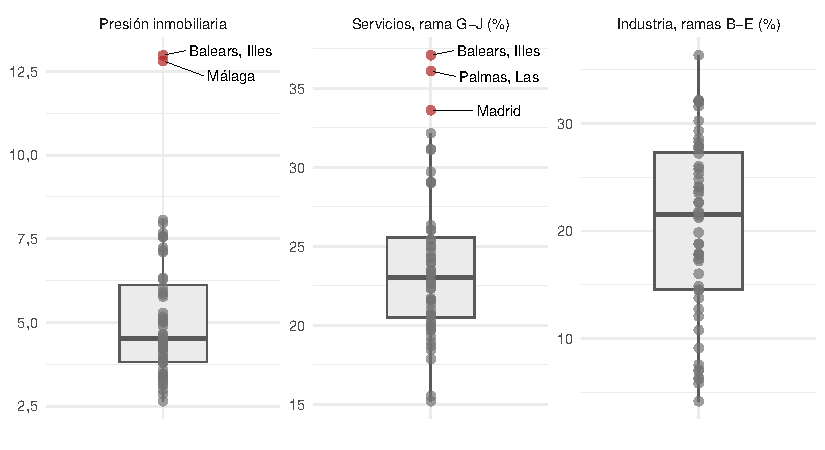
\includegraphics[width=1\linewidth]{ProyectoAEDrticle_files/figure-latex/figatipicos-1} 

}

\caption{Diagramas de caja de las tres variables de análisis; en rojo, las provincias atípicas.\label{fig:atipicos}}\label{fig:figatipicos}
\end{figure}

La presión inmobiliaria presenta dos valores atípicos por la parte alta,
Illes Balears (12,98) y Málaga (12,82), que superan ampliamente la valla
de 9,58 y se separan de la siguiente provincia, Santa Cruz de Tenerife,
con un índice en torno a 8. En el peso de los servicios resultan
atípicas Illes Balears (37,1 \%), Las Palmas (36,1 \%) y Madrid (33,6
\%), esta última por un margen muy estrecho sobre la valla de 33,2 \%.
En cambio, el peso de la industria no presenta ninguna provincia atípica
según este criterio. Ceuta y Melilla son las provincias menos
industrializadas, pero no quedan señaladas, ya que la valla inferior es
negativa y el porcentaje no puede serlo.

\textbf{Decisión:} no se elimina ninguna provincia. Los atípicos son
valores reales, no errores de datos, y además son precisamente los casos
que motivan la pregunta de investigación. Illes Balears resulta atípica
a la vez en presión inmobiliaria y en peso de los servicios, lo que
refleja el patrón que se quiere contrastar, no una anomalía de medición.
Madrid supera la valla de los servicios por un margen muy estrecho (0,4
puntos), por lo que su condición de atípico es débil; aun así se trata
aparte por la singularidad de su PIB per cápita, que refleja el efecto
sede de las empresas. Excluir estos casos eliminaría de la muestra la
evidencia que se quiere contrastar. Por ello empleamos la correlación de
Spearman, que se basa en rangos y es poco sensible a valores extremos, y
comprobamos en la sección de robustez que los resultados se mantienen al
excluir los casos estructuralmente singulares: Madrid, y Ceuta y
Melilla, ciudades pequeñas sin hinterland.

\subsection{Métodos estadísticos}\label{muxe9todos-estaduxedsticos}

Dado el tamaño muestral (52 provincias), la asimetría de las
distribuciones y la presencia de valores atípicos, medimos la asociación
entre variables con el coeficiente de correlación de Spearman, basado en
rangos, y contrastamos su significación (H0: ρ = 0) al nivel del 5 \%.
Para evaluar la robustez de los resultados repetimos el cálculo
excluyendo: Ceuta y Melilla (ciudades autónomas sin hinterland), Madrid
(efecto sede de las empresas), Illes Balears y Málaga (los dos valores
atípicos de presión inmobiliaria) y las cinco a la vez. Como el peso de
los servicios y el de la industria son porcentajes del mismo valor
añadido bruto y están correlacionados entre sí, calculamos también la
correlación parcial de Spearman de cada uno con la presión, controlando
por el otro. Todos los resultados describen asociaciones transversales y
no se interpretan como efectos causales. El análisis se realizó con R y
el ecosistema tidyverse.

\section{Resultados}\label{resultados}

\subsection{Análisis univariante}\label{anuxe1lisis-univariante}

La Tabla \ref{tab:tabdescriptiva} resume la distribución de las cinco
variables y la Figura \ref{fig:hist} muestra su forma.

\begin{table}[H]
\centering
\caption{\label{tab:tabdescriptiva}Estadísticos descriptivos de las variables de análisis (52 provincias, 2022).}
\centering
\fontsize{8}{10}\selectfont
\begin{tabular}[t]{lrrrrrr}
\toprule
Variable & Media & Mediana & DT & Mín. & Máx. & Asimetría\\
\midrule
PIB per cápita (€) & 27.014,23 & 26.316,00 & 5.150,16 & 18.859,00 & 39.246,00 & 0,46\\
Valor medio vivienda (€) & 139.816,68 & 118.794,30 & 64.080,80 & 74.301,10 & 402.810,95 & 1,90\\
Presión inmobiliaria & 5,21 & 4,52 & 2,16 & 2,65 & 12,98 & 1,74\\
Servicios, G-J (\%) & 23,80 & 23,04 & 4,80 & 15,20 & 37,09 & 0,83\\
Industria, B-E (\%) & 20,38 & 21,51 & 8,36 & 4,14 & 36,36 & -0,24\\
\bottomrule
\end{tabular}
\end{table}

\begin{figure}[H]

{\centering 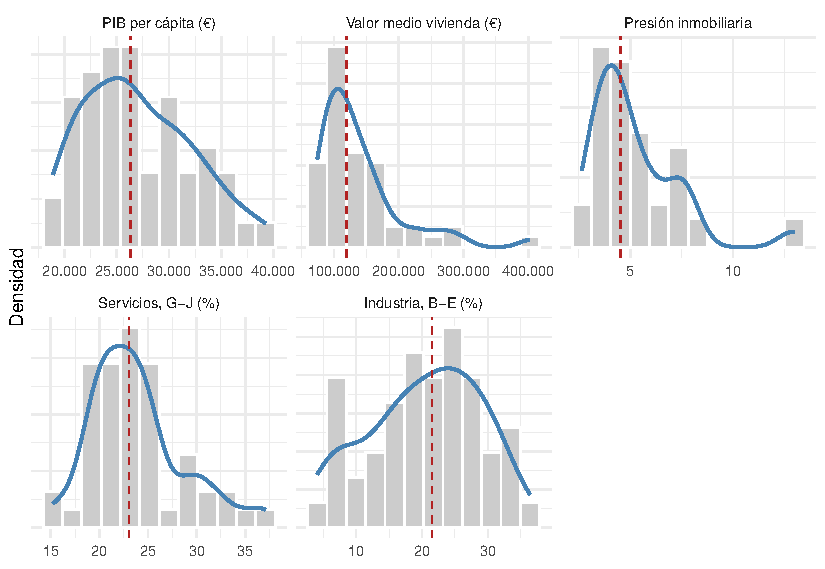
\includegraphics[width=1\linewidth]{ProyectoAEDrticle_files/figure-latex/fighist-1} 

}

\caption{Distribución de las variables de análisis: histograma, densidad (azul) y mediana (rojo discontinuo).\label{fig:hist}}\label{fig:fighist}
\end{figure}

Los resultados muestran tres rasgos. En primer lugar, el PIB per cápita
es la variable más homogénea: la media (27.014 €) y la mediana (26.316
€) son próximas, la asimetría es moderada (0,46) y el coeficiente de
variación ronda el 19 \%. Los valores van desde 18.859 € en Jaén hasta
39.246 € en Madrid, seguida de Araba/Álava y Gipuzkoa.

En segundo lugar, el valor medio de la vivienda es mucho más desigual
que la riqueza. Su media (139.817 €) supera con claridad a la mediana
(118.794 €) y la distribución presenta una cola larga hacia la derecha
(asimetría de 1,90), con Illes Balears (402.811 €), Madrid (297.801 €) y
Málaga (275.159 €) en el extremo. Entre la provincia más cara y la más
barata, Ciudad Real (74.301 €), la vivienda se multiplica por 5,4,
mientras que el PIB per cápita solo lo hace por 2,1. Esta diferencia de
dispersión es coherente con la idea del espejismo: el precio de la
vivienda varía mucho más que la riqueza que genera cada provincia.

En tercer lugar, la presión inmobiliaria hereda esa asimetría positiva
(1,74). El valor medio de una vivienda equivale en la provincia mediana
a 4,5 veces el PIB per cápita, y la mitad de las provincias se sitúa
entre 3,8 y 6,1; en cambio, Illes Balears y Málaga superan 12,8, más del
doble de la mediana. La estructura productiva es más equilibrada: el
peso de los servicios tiene una cola derecha moderada (asimetría de
0,83) debida a Illes Balears, Las Palmas y Madrid, y el de la industria
es casi simétrico (−0,24), con una gran dispersión que va del 4,1 \% de
Melilla al 36,4 \% de Guadalajara.

El histograma de la presión inmobiliaria revela además un segundo grupo
en torno a 7-8, formado por territorios de naturaleza muy distinta:
islas turísticas (Santa Cruz de Tenerife, Las Palmas), grandes capitales
(Madrid, Barcelona), ciudades autónomas (Ceuta, Melilla) y también Cádiz
y Gipuzkoa. Es un primer indicio de que una presión elevada no responde
a una única causa, algo que se analiza en el apartado siguiente. La
distribución de la industria presenta, por su parte, un pequeño grupo de
provincias por debajo del 10 \% (entre ellas Melilla, Ceuta, Almería y
Málaga) que genera un ligero hombro por la izquierda.

Estas asimetrías, junto con los atípicos del apartado anterior,
respaldan el uso de correlaciones basadas en rangos en lugar de la
correlación de Pearson.

\subsection{Análisis bivariante: el espejismo del
PIB}\label{anuxe1lisis-bivariante-el-espejismo-del-pib}

La Tabla \ref{tab:tabtop10} recoge las diez provincias con mayor presión
inmobiliaria.

\begin{table}[H]
\centering
\caption{\label{tab:tabtop10}Las diez provincias con mayor presión inmobiliaria, 2022.}
\centering
\fontsize{8}{10}\selectfont
\begin{tabular}[t]{lrrrrr}
\toprule
Provincia & PIB pc (€) & Vivienda (€) & Presión & Servicios (\%) & Industria (\%)\\
\midrule
Balears, Illes & 31.030 & 402.811 & 12,98 & 37,1 & 7,0\\
Málaga & 21.470 & 275.159 & 12,82 & 29,1 & 6,3\\
Santa Cruz de Tenerife & 22.108 & 178.237 & 8,06 & 32,1 & 7,1\\
Melilla & 19.433 & 154.903 & 7,97 & 19,3 & 4,1\\
Palmas, Las & 22.358 & 171.641 & 7,68 & 36,1 & 7,5\\
\addlinespace
Madrid & 39.246 & 297.801 & 7,59 & 33,6 & 9,1\\
Cádiz & 20.644 & 156.165 & 7,56 & 23,5 & 17,9\\
Ceuta & 21.273 & 160.747 & 7,56 & 21,7 & 5,8\\
Gipuzkoa & 36.374 & 263.246 & 7,24 & 22,8 & 26,0\\
Barcelona & 33.270 & 237.844 & 7,15 & 29,0 & 18,8\\
\bottomrule
\end{tabular}
\end{table}

Siete de las diez tienen un peso de servicios superior a la mediana
nacional (23,0 \%), y las dos primeras, Illes Balears y Málaga, destacan
con diferencia. Sin embargo, el ranking no es una lista de destinos
turísticos: incluye grandes capitales (Madrid y Barcelona), las dos
ciudades autónomas (Melilla y Ceuta), Cádiz y una provincia industrial,
Gipuzkoa, con un 26,0 \% de industria.

La Figura \ref{fig:espejismo} enfrenta el PIB per cápita con el valor
medio de la vivienda y colorea cada provincia según el peso de la rama
G-J.

\begin{figure}[H]

{\centering 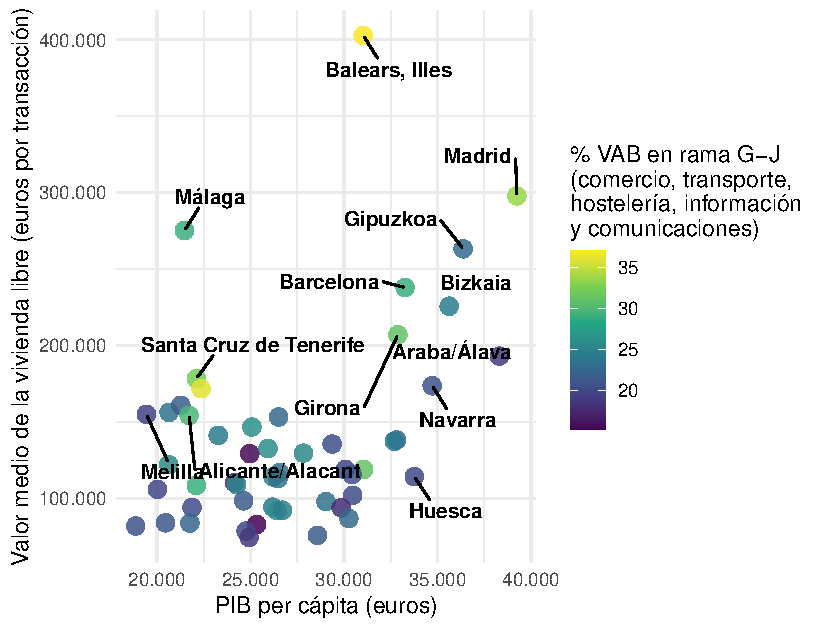
\includegraphics[width=1\linewidth]{ProyectoAEDrticle_files/figure-latex/grafico-espejismo-1} 

}

\caption{El espejismo del PIB: PIB per cápita y valor medio de la vivienda por provincia, 2022. Fuente: elaboración propia con datos del INE y del Ministerio de Vivienda.\label{fig:espejismo}}\label{fig:grafico-espejismo}
\end{figure}

La correlación de Spearman entre el PIB per cápita y el valor medio de
la vivienda es débil (ρ = 0,29, p = 0,036): la riqueza provincial
explica poco del nivel de precios. Si estos siguieran a la renta local,
la vivienda sería mucho más cara en las provincias más ricas y la
presión inmobiliaria sería similar en todas. Lo que se observa es que el
precio varía mucho más (coeficiente de variación del 46 \%) que el PIB
per cápita (19 \%), y que una presión alta aparece tanto en provincias
de PIB bajo (Málaga, Melilla) como alto (Madrid, Gipuzkoa), sin relación
significativa con la riqueza (ρ = -0,18, p = 0,21).

Los casos que más se desvían son Illes Balears y Málaga. Illes Balears
combina el mayor peso de servicios (37,1 \%) con el precio más alto
(402.811 €) y un PIB per cápita de 31.030 €, algo por encima de la
mediana. Málaga, con un 29,1 \% de servicios, alcanza 275.159 € con un
PIB per cápita de solo 21.470 €.

En el extremo derecho, Madrid, Araba/Álava y Gipuzkoa tienen los PIB per
cápita más altos, pero con estructuras muy distintas. El País Vasco no
escapa a una presión elevada pese a su perfil industrial: Araba/Álava
(5,04), Bizkaia (6,33) y Gipuzkoa (7,24) están por encima de la mediana
nacional (4,52). Madrid (7,59) y Barcelona (7,15) combinan PIB y precios
altos y figuran entre las diez provincias de mayor presión, de modo que
un PIB elevado no basta para evitar una vivienda cara en relación con la
renta.

\subsection{Servicios, industria y presión
inmobiliaria}\label{servicios-industria-y-presiuxf3n-inmobiliaria}

La Figura \ref{fig:bivar} enfrenta el peso de cada sector con la presión
inmobiliaria y la Tabla \ref{tab:tabterciles} compara la presión mediana
entre grupos de provincias.

\begin{figure}[H]

{\centering 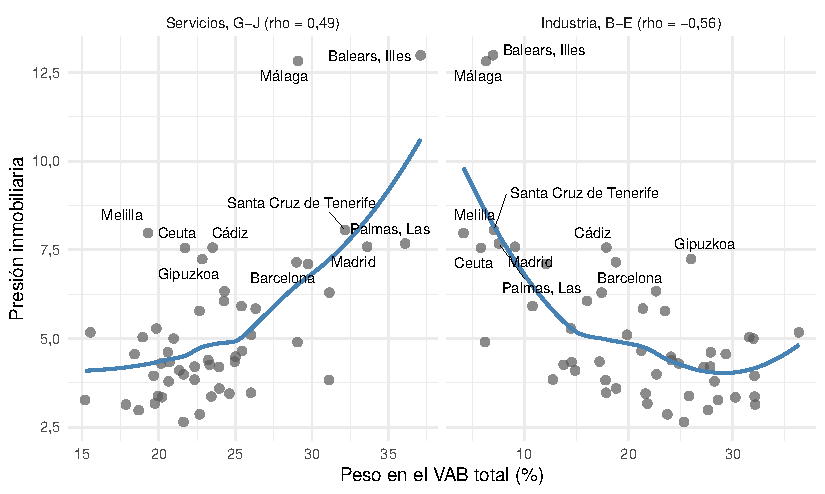
\includegraphics[width=1\linewidth]{ProyectoAEDrticle_files/figure-latex/figbivar-1} 

}

\caption{Presión inmobiliaria según el peso de los servicios y de la industria. Línea: ajuste local (loess). Se etiquetan las diez provincias de mayor presión.\label{fig:bivar}}\label{fig:figbivar}
\end{figure}

\begin{table}[H]
\centering
\caption{\label{tab:tabterciles}Presión inmobiliaria mediana según el tercil de peso de cada sector.}
\centering
\fontsize{8}{10}\selectfont
\begin{tabular}[t]{llrrrr}
\toprule
Estructura & Tercil & n & Peso mín. (\%) & Peso máx. (\%) & Presión mediana\\
\midrule
Servicios (G-J) & Bajo & 18 & 15,20 & 21,36 & 4,20\\
Servicios (G-J) & Medio & 17 & 21,61 & 24,62 & 4,21\\
Servicios (G-J) & Alto & 17 & 24,97 & 37,09 & 5,91\\
Industria (B-E) & Bajo & 18 & 4,14 & 17,42 & 6,18\\
Industria (B-E) & Medio & 17 & 17,79 & 24,81 & 4,39\\
\addlinespace
Industria (B-E) & Alto & 17 & 25,32 & 36,36 & 3,95\\
\bottomrule
\end{tabular}
\end{table}

\textbf{Servicios.} El peso de los servicios se asocia de forma positiva
y moderada con la presión inmobiliaria (ρ = 0,49), pero la relación no
es homogénea. La presión mediana es prácticamente idéntica en el tercil
bajo (4,20) y en el medio (4,21) y solo aumenta en el alto (5,91): la
asociación se concentra en las provincias más terciarizadas, entre ellas
Illes Balears, Las Palmas, Santa Cruz de Tenerife y Málaga. La curva de
la figura es plana hasta aproximadamente el 25 \% de servicios y
asciende con fuerza a partir de ese punto, de modo que la asociación no
es lineal.

\textbf{Industria.} El peso de la industria presenta una asociación
negativa de magnitud similar (ρ = -0,56), pero también aquí se concentra
en un extremo: la presión mediana cae de 6,18 en el tercil menos
industrial a 4,39 en el medio y apenas varía en el tercil más industrial
(3,95). La curva de la Figura \ref{fig:bivar} confirma que el descenso
se produce sobre todo por debajo del 15-20 \% de industria, a partir del
cual la presión se estabiliza en torno a 4-5. Las provincias con menor
peso industrial, como Illes Balears, Málaga, Santa Cruz de Tenerife, Las
Palmas, Madrid, Melilla o Ceuta, son las de presión más alta.

\textbf{Excepciones.} El patrón admite excepciones relevantes. Melilla y
Ceuta tienen una presión alta con un peso de servicios cercano al de la
media (19,3 \% y 21,7 \%), y Gipuzkoa y Barcelona la tienen con perfiles
industriales. En el extremo contrario, las provincias de menor presión
(Cuenca, Teruel, Ciudad Real, Palencia, Zamora o Cáceres) son
interiores, con poco peso de servicios y, en general, una industria
apreciable.

Estos resultados describen asociaciones y no permiten atribuir el nivel
de presión a la estructura productiva. Además, servicios e industria se
mueven en sentido contrario (se analiza en el apartado de robustez), y
buena parte de las provincias menos industriales coincide con las más
terciarizadas, por lo que sus efectos no pueden separarse con estos
datos.

\subsection{Robustez de los
resultados}\label{robustez-de-los-resultados}

La Tabla \ref{tab:tabrobustez} recoge las correlaciones de Spearman en
la muestra completa y en cuatro submuestras.

\begin{table}[H]
\centering
\caption{\label{tab:tabrobustez}Correlaciones de Spearman con la presión inmobiliaria y robustez a la exclusión de provincias singulares.}
\centering
\fontsize{8}{10}\selectfont
\begin{tabular}[t]{lrrrrrr}
\toprule
Muestra & n & $\rho$ servicios & p  & $\rho$ industria & p & $\rho$ serv.-ind.\\
\midrule
Todas las provincias & 52 & 0,49 & $<$0,001 & -0,56 & $<$0,001 & -0,62\\
Sin Ceuta y Melilla & 50 & 0,57 & $<$0,001 & -0,51 & $<$0,001 & -0,73\\
Sin Madrid & 51 & 0,46 & $<$0,001 & -0,53 & $<$0,001 & -0,60\\
Sin Illes Balears y Málaga & 50 & 0,43 & 0,002 & -0,51 & $<$0,001 & -0,59\\
Sin las cinco anteriores & 47 & 0,48 & $<$0,001 & -0,41 & 0,004 & -0,68\\
\bottomrule
\end{tabular}
\end{table}

Con las 52 provincias, la presión inmobiliaria muestra una correlación
moderada y positiva con el peso de los servicios (ρ = 0,49) y moderada y
negativa con el peso de la industria (ρ = -0,56), ambas con p
\textless{} 0,001. Las dos asociaciones \textbf{se mantienen en todas
las submuestras}: sin Ceuta y Melilla la de servicios aumenta (0,57);
sin Madrid (0,46) o sin Illes Balears y Málaga (0,43) se reduce algo
pero sigue siendo significativa; y al excluir a la vez las cinco
provincias singulares los valores son 0,48 en servicios y -0,41 en
industria. Ningún caso aislado explica, por tanto, los resultados.

\textbf{Efecto conjunto.} El peso de la industria y el de los servicios
están fuertemente correlacionados entre sí (entre -0,73 y -0,59), como
cabe esperar al ser porcentajes del mismo VAB. Para separar sus
contribuciones calculamos la correlación parcial de Spearman. Al
controlar por la industria, la asociación de la presión con los
servicios cae a ρ = 0,22 y deja de ser significativa (p = 0,12),
mientras que la asociación con la industria, controlando por los
servicios, se mantiene (ρ = -0,37, p = 0,007).

\section{Discusión}\label{discusiuxf3n}

\subsection{Interpretación de los
resultados}\label{interpretaciuxf3n-de-los-resultados}

El análisis arroja dos hallazgos distintos. El primero se refiere al
espejismo del PIB: la riqueza provincial explica poco del precio de la
vivienda (ρ = 0,29) y no guarda relación significativa con la presión
inmobiliaria (ρ = -0,18, p = 0,21). El valor de la vivienda varía más
del doble que el PIB per cápita (coeficientes de variación del 46 \% y
el 19 \%), y una presión alta aparece tanto en provincias de PIB bajo,
como Málaga o Melilla, como alto, como Madrid o Gipuzkoa. El PIB per
cápita, por sí solo, no permite anticipar cuánto cuesta la vivienda en
relación con la renta de un territorio.

El segundo hallazgo se refiere a la estructura productiva. La presión
inmobiliaria se asocia positivamente con el peso de los servicios (ρ =
0,49) y negativamente con el de la industria (ρ = -0,56), y ambas
asociaciones resisten la exclusión de Ceuta y Melilla, de Madrid, de
Illes Balears y Málaga, y de las cinco a la vez. Las dos tienen además
una forma no lineal: la presión solo se eleva de manera apreciable en el
tercio de provincias más terciarizadas (mediana de 5,91 frente a 4,20 y
4,21 en los otros dos) y es claramente mayor en el tercio menos
industrial (6,18 frente a 4,39 y 3,95).

Sin embargo, estos resultados no permiten atribuir la presión
específicamente a los servicios. La razón es en parte estadística:
servicios e industria son porcentajes del mismo VAB y están fuertemente
correlacionados entre sí, de modo que, descontada la industria, la
asociación con los servicios es pequeña y no significativa (ρ parcial =
0,22, p = 0,12), mientras que la de la industria se mantiene (ρ parcial
= -0,37, p = 0,007). Y en parte es de medición, porque la rama G-J
agrupa hostelería con comercio, transporte, información y
comunicaciones, y no aísla la dependencia turística. Por último, el
patrón admite excepciones: Ceuta y Melilla presentan una presión elevada
sin un peso de servicios destacado, y Gipuzkoa y Barcelona la presentan
con perfiles industriales, lo que indica que hay otros factores en
juego.

\subsection{Limitaciones}\label{limitaciones}

\begin{itemize}
\tightlist
\item
  \textbf{Medición del turismo.} La variable de servicios es una
  aproximación amplia. Una parte del peso de G-J en provincias como
  Madrid puede deberse a actividades no turísticas.
\item
  \textbf{PIB y vivienda.} El PIB provincial mide la actividad producida
  en el territorio, no la renta de sus residentes, y está sujeto al
  efecto sede en Madrid. El valor medio por transacción depende además
  del tipo y tamaño de las viviendas vendidas, y no equivale a un precio
  por metro cuadrado.
\item
  \textbf{Casos singulares.} Ceuta y Melilla son ciudades pequeñas sin
  hinterland, por lo que su comparación con provincias es discutible. Se
  verificó que excluirlas no altera las conclusiones.
\item
  \textbf{Diseño.} Se trata de un corte transversal de un solo año y 52
  observaciones, con potencia limitada, que describe asociaciones entre
  agregados provinciales y no permite inferir causalidad ni extrapolar a
  individuos u hogares. Las correlaciones parciales se calcularon sobre
  rangos y sus p-valores son aproximados.
\end{itemize}

Como líneas futuras, convendría desagregar la hostelería de las demás
ramas, incorporar precios de alquiler, ampliar el análisis a varios años
y considerar otras variables, como el saldo migratorio joven.

\section{Conclusiones}\label{conclusiones}

\textbf{El espejismo del PIB.} Los datos respaldan que el PIB per cápita
provincial es un indicador insuficiente para valorar la presión que
soporta el mercado de la vivienda. Su relación con el valor de la
vivienda es débil (ρ = 0,29), la presión inmobiliaria no está
significativamente asociada a él, y las provincias con mayor presión,
Illes Balears (12,98) y Málaga (12,82), triplican aproximadamente la
mediana nacional (4,52) con niveles de PIB muy dispares entre sí.

\textbf{La trampa turística.} La hipótesis se confirma solo en parte.
Las provincias con más peso de servicios tienden a soportar mayor
presión inmobiliaria (ρ = 0,49) y las más industrializadas, menor (ρ =
-0,56), y ambas asociaciones son robustas a la exclusión de provincias
singulares. Pero la asociación con los servicios no se sostiene al
controlar por el peso de la industria, y la variable disponible no
distingue el turismo del resto de servicios, por lo que no podemos
afirmar que la especialización turística, en sentido estricto, sea la
causa de la presión. Lo que los datos muestran es que el mayor coste de
la vivienda en relación con la renta se concentra en las provincias
terciarizadas y poco industriales, con excepciones relevantes.

Estas conclusiones describen asociaciones transversales de 2022 en 52
provincias y no deben interpretarse como relaciones causales.

%%%%%%%%%%%%%%%%%%%%%%%%%%%%%%%%%%%%%%%%%%

\vspace{6pt}

%%%%%%%%%%%%%%%%%%%%%%%%%%%%%%%%%%%%%%%%%%
%% optional

% Only for the journal Methods and Protocols:
% If you wish to submit a video article, please do so with any other supplementary material.
% \supplementary{The following supporting information can be downloaded at: \linksupplementary{s1}, Figure S1: title; Table S1: title; Video S1: title. A supporting video article is available at doi: link.}

%%%%%%%%%%%%%%%%%%%%%%%%%%%%%%%%%%%%%%%%%%







%%%%%%%%%%%%%%%%%%%%%%%%%%%%%%%%%%%%%%%%%%
%% Optional

%% Only for journal Encyclopedia


%%%%%%%%%%%%%%%%%%%%%%%%%%%%%%%%%%%%%%%%%%
%% Optional
%%%%%%%%%%%%%%%%%%%%%%%%%%%%%%%%%%%%%%%%%%
\begin{adjustwidth}{-\extralength}{0cm}

%\printendnotes[custom] % Un-comment to print a list of endnotes



% If authors have biography, please use the format below
%\section*{Short Biography of Authors}
%\bio
%{\raisebox{-0.35cm}{\includegraphics[width=3.5cm,height=5.3cm,clip,keepaspectratio]{Definitions/author1.pdf}}}
%{\textbf{Firstname Lastname} Biography of first author}
%
%\bio
%{\raisebox{-0.35cm}{\includegraphics[width=3.5cm,height=5.3cm,clip,keepaspectratio]{Definitions/author2.jpg}}}
%{\textbf{Firstname Lastname} Biography of second author}

%%%%%%%%%%%%%%%%%%%%%%%%%%%%%%%%%%%%%%%%%%
%% for journal Sci
%\reviewreports{\\
%Reviewer 1 comments and authors’ response\\
%Reviewer 2 comments and authors’ response\\
%Reviewer 3 comments and authors’ response
%}
%%%%%%%%%%%%%%%%%%%%%%%%%%%%%%%%%%%%%%%%%%
\PublishersNote{}
\end{adjustwidth}


\end{document}
